\documentclass[border=4pt]{standalone}
\usepackage{tikz}
\usetikzlibrary{arrows.meta}
\begin{document}
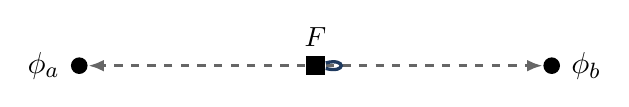
\begin{tikzpicture}[scale=1.0, every node/.style={inner sep=0pt}]
  \tikzset{ext/.style={circle, inner sep=0pt, minimum size=6.0pt, fill=black}}
  \tikzset{vert/.style={rectangle, inner sep=0pt, minimum size=7.0pt, fill=black}}
  \tikzset{C/.style={draw={rgb,255:red,31;green,58;blue,95}, solid, line width=1.2pt}}
  \tikzset{R/.style={draw={rgb,255:red,102;green,102;blue,102}, dashed, line width=1.2pt, -{Latex[length=2mm]}}}
  \node[ext, label={[label distance=3.7pt,font=\fontsize{11.0}{13.2}\selectfont]left:$\phi_{a}$}] (ext0) at (-3.0000, 0.0000) {};
  \node[ext, label={[label distance=3.7pt,font=\fontsize{11.0}{13.2}\selectfont]right:$\phi_{b}$}] (ext1) at (3.0000, 0.0000) {};
  \node[vert, label={[label distance=3.0pt,font=\fontsize{10.0}{12.0}\selectfont]above:$F$}] (vert2) at (0.0000, 0.0000) {};
  % propagators
  \draw[R] (vert2) -- (ext0);
  \draw[R] (vert2) -- (ext1);
  \draw[C] (vert2) edge[loop right, looseness=10] (vert2);
\end{tikzpicture}
\end{document}
